\documentclass{beamer}

\mode<presentation> {
\usetheme{Madrid}
}

\usepackage{graphicx}
\usepackage{booktabs}
\usepackage{polski}
\usepackage[polish]{babel}
\usepackage[utf8]{inputenc}
\usepackage[T1]{fontenc}
\usepackage[utf8]{luainputenc}
\usepackage{pgfgantt}
\usepackage{caption}
\usepackage{mwe}

% Strona tytułowa
\usepackage{pgfplots}
\usepackage{siunitx}
\usepackage{paracol}
\usepackage{gensymb}

% Pływające obrazki
\usepackage{float}
\usepackage{svg}
\usepackage{graphicx}
\usepackage{subfig}


\sisetup{group-digits=true,
        %  group-four-digits=true,
        round-precision=4,
        group-separator={},
        output-decimal-marker={,}}

\DeclareCaptionFormat{citation}{%
   \ifx\captioncitation\relax\relax\else
     \captioncitation\par
   \fi
   #1#2#3\par}
\newcommand*\setcaptioncitation[1]{\def\captioncitation{\tiny{\textit{Źródło:}~#1}\medskip}\normalsize}
\let\captioncitation\relax
\captionsetup{format=citation,justification=centering}

\usetikzlibrary{pgfplots.groupplots}
\sisetup{detect-weight,exponent-product=\cdot,output-decimal-marker={,},per-mode=symbol,binary-units=true,range-phrase={-},range-units=single}

%wymiar tekstu
\def\figurename{Rys.}
\def\tablename{Tab.}

%----------------------------------------------------------------------------------------
%	TITLE PAGE
%----------------------------------------------------------------------------------------

\title[WEDT - Projekt]{Wprowadzenie do eksploracji danych tekstowych w~sieci~WWW}

\author[Konieczka, Poturała, Sikora]{Maria Konieczka \and Alicja Poturała \and Jakub Sikora} 

\date{3 czerwca 2020}
\institute[]{Odpowiadanie na pytania ogólne zadane w~języku polskim}

\AtBeginSection[]
{
    \begin{frame}[plain, noframenumbering]
        \frametitle{Agenda}
        \tableofcontents[currentsection]
    \end{frame}
}

\begin{document}

\begin{frame}
\titlepage
\end{frame}

\begin{frame}
  \frametitle{Agenda}
  \tableofcontents
\end{frame}

\section{Wprowadzenie w problem}

\begin{frame}
  \frametitle{Definicja zadania}
  \begin{block}{Zadanie odpowiadania na pytania}
    Zadanie odpowiadania na pytania polega na automatycznej \begin{itemize}
      \item analizie otrzymanego pytania w~języku naturalnym,
      \item wyszukiwaniu odpowiednich dokumentów,
      \item ekstrakcji wiedzy,
      \item generacji odpowiedzi, również w~języku naturalnym. 
    \end{itemize}
  \end{block}
\end{frame}

\begin{frame}
  \frametitle{Założenia systemu}
  \begin{block}{Główne założenia systemu:}
  \begin{itemize}
    \item pytania zadawane są w~języku polskim,
    \item system analizuje wiedzę zapisaną w~postaci podsumowań wyników wyszukiwarek internetowych,
    \item system odpowiada na zamknięty zestaw kategorii (domen),
    \item system odpowiada w~postaci jednego do trzech wyrazów, nie zajmujemy się generacją zdań.
  \end{itemize}
\end{block}
\end{frame}

\section{Algorytm wyszukiwania odpowiedzi}
\begin{frame}
  \frametitle{Ogólny opis algorytmu wyszukiwania}
  \bigskip
  \begin{figure}
    \centering
    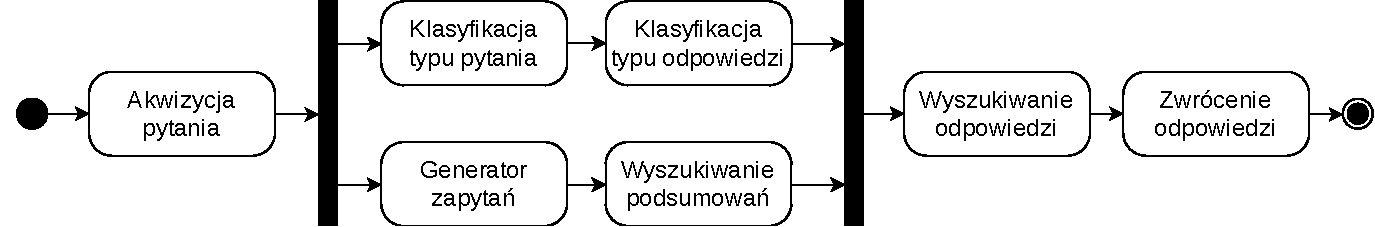
\includegraphics[width=\columnwidth]{figures/WEDT-Algorytm-Rotated.pdf}
    \caption{Ogólny schemat blokowy algorytmu wyszukiwania odpowiedzi}
    \label{fig:ir-algorytm}
  \end{figure}
\end{frame}

\begin{frame}
  \frametitle{Akwizycja pytania}
    \begin{itemize}
      \item zadawanie pytań odbywa się poprzez dedykowany interfejs graficzny, bądź specjalne REST API,
      \item każde pytanie jest analizowane w sposób indywidualny, bez przechowywania wcześniejszych pytań i utrzymywania kontekstu,
      \item nie zakładamy również żadnego profilowania użytkowników, ponieważ typowe pytania o fakty, są ze sobą słabo powiązane,
      \item przy zadaniu każdego pytania użytkownik może wybrać strategię i silnik wyszukiwania.
    \end{itemize}
\end{frame}

\begin{frame}
  \frametitle{Generacja zapytań}
  Generacja zapytań to proces wytwarzania specjalnych zapytań do wyszukiwarki, w~zależności od obranej strategii. W~projekcie zaimplementowane zostały trzy strategie:
  \begin{itemize}
    \item singlequery,
    \item stopwords,
    \item chunks.
  \end{itemize}
  Wytworzenie kilku zapytań z~jednego pytania, zwiększa bazę zebranych podsumowań.
\end{frame}

\begin{frame}
  \frametitle{Wyszukiwanie podsumowań}
  Przygotowany zbiór zapytań jest wykorzystywany przez \textit{webscrapowaniu} stron popularnych wyszukiwarek internetowych. System emuluje zachowanie przeglądarki Firefox, pobiera i~renderuje dokument HTML, następnie wycina z~dokumentu wszystkie interesujące podsumowania.
  System obsługuje kilka wyszukiwarek internetowych:
  \begin{itemize}
    \item google,
    \item yahoo,
    \item bing,
    \item duckduckgo.
  \end{itemize}
\end{frame}

\begin{frame}
  \frametitle{Klasyfikacja typu pytania}
  W~międzyczasie, system dokonuje klasyfikacji typu pytania. Wyróżniamy 16 typów pytań. Klasyfikacja typu pytania odbywa się przy użyciu wyrażeń regularnych wyszukujących zaimki pytające, związane z~danym typem. Docelowo, typ pytania będzie potrzebny do określenia jednego z~typów odpowiedzi:
  \begin{itemize}
    \item \texttt{DATA},
    \item \texttt{MIEJSCE},
    \item \texttt{WIELKOŚĆ},
    \item \texttt{OSOBA},
    \item \texttt{RZECZ}.
  \end{itemize}
\end{frame}

\begin{frame}
  \frametitle{Klasyfikacja typu odpowiedzi}
  Na podstawie typu pytania, określany jest typ odpowiedzi. W~przypadku oczywistych typów pytań, jeden zaimek pytający odpowiada jednemu typowi odpowiedzi. 
  \begin{center}
    \textit{czyj?} --- \texttt{OSOBA}
  \end{center}
  Dla niektórych typów pytań, nie da się jednoznacznie określić typu odpowiedzi. W~takim przypadku korzystamy z~listy możliwych typów odpowiedzi.
  \begin{center}
    \textit{jak?} --- \texttt{[WIELKOŚĆ, OSOBA, MIEJSCE, RZECZ]}
  \end{center}
\end{frame}

\begin{frame}
  \frametitle{Wyszukiwanie odpowiedzi}
  Każde otrzymane podsumowanie przetwarzane jest narzędziem \textit{tagger}, w~celu zamiany słów na odpowiadające im leksemy. Następnie, w~zależności od oczekiwanego typu odpowiedzi,
  na podsumowaniach stosowane są albo wyrażenia regularne albo podział na n-gramy i~filtracja względem częstości.
\end{frame}

\begin{frame}
  \frametitle{Zwrócenie odpowiedzi}
  Wraz z~uzyskaną odpowiedzią, użytkownikowi zwracany jest link do dokumentu, którego podsumowanie ostatecznie zwróciło odpowiedź. Jeżeli użytkownik korzystał z~dedykowanego interfejsu graficznego, może wrócić do strony głównej i~zadać pytanie jeszcze raz.
\end{frame}

\section{Implementacja i korzystanie z systemu}
\begin{frame}
  \frametitle{Architektura mikroserwisowa}
  \begin{figure}
    \centering
    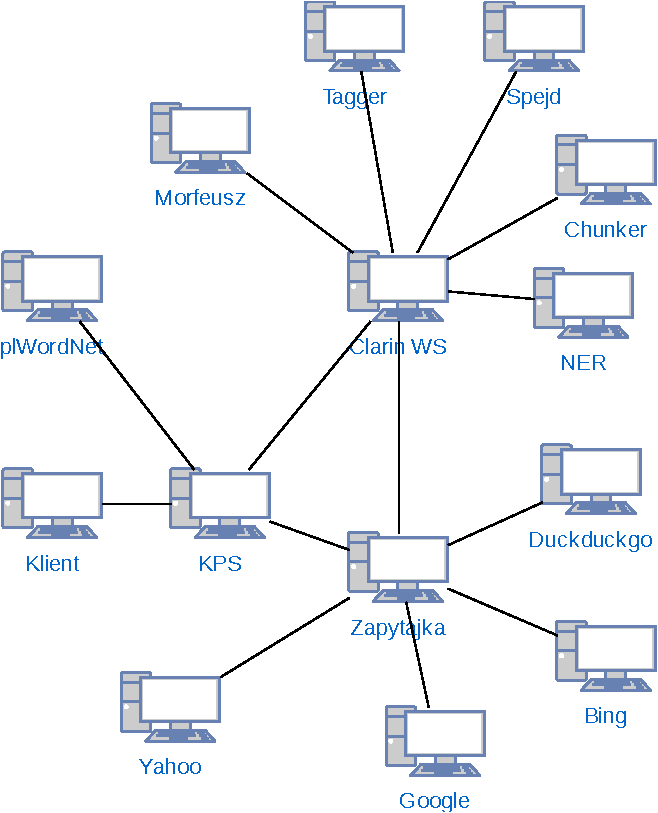
\includegraphics[width=0.5\columnwidth]{figures/WEDT-Uslugi.pdf}
    \label{fig:klient}
  \end{figure}
\end{frame}

\begin{frame}
  \frametitle{Implementacja systemu}
  \begin{block}{Implementacja modułów:}
    \begin{itemize}
      \item odpowiadania na pytania,
      \item klienta internetowego,
      \item \textit{webscrapera} wyszukiwarek internetowych.
    \end{itemize}
  \end{block}

  \begin{block}{Integracja z usługami:}
    \begin{itemize}
      \item plWordNet,
      \item CLARIN WS
      \begin{itemize}
        \item morfeusz,
        \item tagger,
        \item spejd,
        \item chunker,
        \item Named-Entity Recognition.
      \end{itemize}
    \end{itemize}
  \end{block}
\end{frame}

\begin{frame}
  \frametitle{Klient systemu} 
  \begin{figure}
    \centering
    \fbox{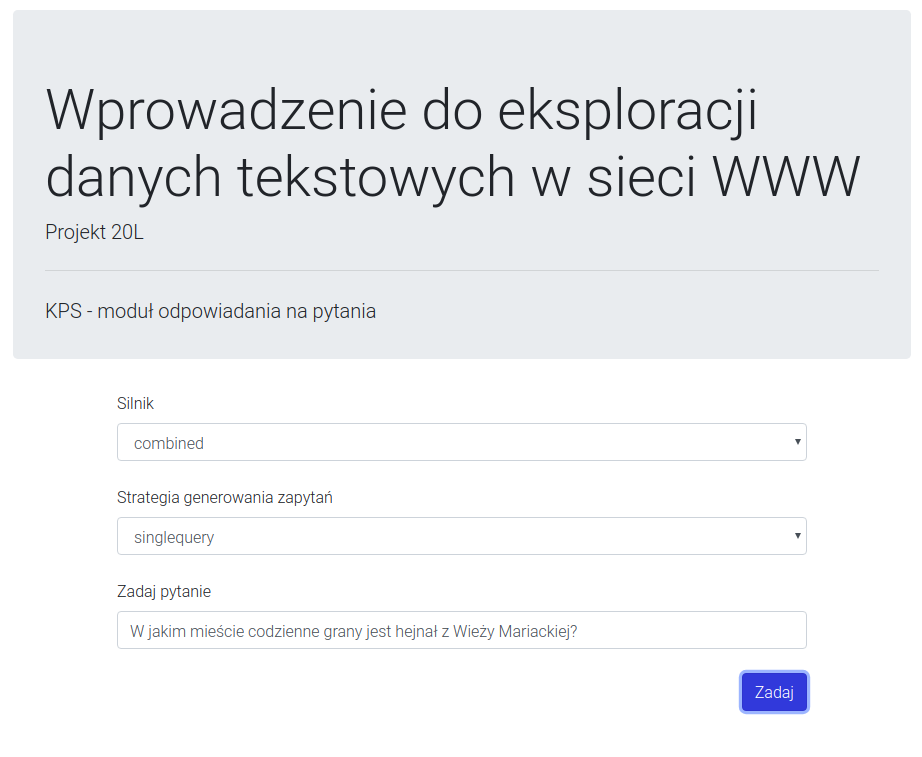
\includegraphics[width=0.7\columnwidth]{figures/kps.png}}
    \label{fig:klient}
  \end{figure}
\end{frame}

\begin{frame}
  \frametitle{Klient systemu} 
  \begin{figure}
    \centering
    \fbox{
\includegraphics[width=0.7\columnwidth]{figures/kps-answer.png}}
    \label{fig:klient-odp}
  \end{figure}
\end{frame}

\section{Wyniki badań}
\begin{frame}
  \frametitle{Badanie wyszukiwarek internetowych}
  \begin{figure}
    \begin{tikzpicture}
        \begin{axis}[
            grid=both,
            width=\columnwidth,
            height=7.5cm,
            ybar,
            ymin=0,
            bar width=0.5cm,
            enlarge x limits=0.2,
            area legend,
            legend style={at={(0.5,-0.15)},
            anchor=north,
            legend columns=2},
            ylabel={Liczba odpowiedzi},
            symbolic x coords={dobra, częściowo, błędna, brak},
            xtick=data,
            nodes near coords,
            x label style={
            fixed},
            ]
        \legend{google, duckduckgo}
        \addplot coordinates {(dobra,80) (częściowo,8) (błędna,137) (brak,31)};
        \addplot coordinates {(dobra,66) (częściowo,3) (błędna,111) (brak,76)};
		\end{axis}
        \end{tikzpicture}
        \label{fig:porownanie-wyszukiwarek}
  \end{figure}
\end{frame}


\begin{frame}
  \frametitle{Badanie wyszukiwarek internetowych}
  \begin{table}[h]
    \centering
    \begin{tabular}{|c|c|c|c|c|c|c|}
      \hline
      \textbf{przeglądarka} & $n_g$ &$n_{pg}$&$n_n$&$n_w$&$cov.$&$prec.$  \\ \hline
      \textit{Google}&80&8&31&137&$\num{0.88}$&$\num{0.36}$ \\ \hline
      \textit{DuckDuckGo}&66&3&76&111&$\num{0.70}$&$\num{0.37}$ \\ \hline
    \end{tabular}
    \caption{Porównanie otrzymanych wyników dla przeglądarek \textit{Google} oraz \textit{DuckDuckGo}}
    
    \label{tab:porownanieWysz}
    
  \end{table}
\end{frame}

\begin{frame}
  \frametitle{Badanie strategii generacji zapytań}
  \begin{figure}
    \begin{tikzpicture}
    \begin{axis}[
    grid=both,
    width=\columnwidth,
    height=7.5cm,
    ybar,
    ymin=0,
    bar width=0.4cm,
    enlarge x limits=0.2,
    area legend,
    legend style={at={(0.5,-0.15)},
      anchor=north,
      legend columns=3},
    ylabel={Liczba odpowiedzi},
    symbolic x coords={dobra, częściowo, błędna, brak},
    xtick=data,
    nodes near coords,
    x label style={
      fixed},
    ]
    \legend{stopwords, singlequery, chunks}
    \addplot coordinates {(dobra,80) (częściowo,8) (błędna,137) (brak,31)};
    \addplot coordinates {(dobra,85) (częściowo,9) (błędna,128) (brak,34)};
    \addplot coordinates {(dobra,57) (częściowo,6) (błędna,105) (brak,88)};
    \end{axis}
    \end{tikzpicture}
    \label{fig:porownanie-strategie}
  \end{figure}
\end{frame}

\section{Wnioski i przemyślenia}
\begin{frame}
  \frametitle{Wnioski z projektu}
  \begin{block}{Wychwytywanie dat}
    Wyrażenia regularne dobrze sprawdzają się przy odpowiadaniu na pytania o~daty.
  \end{block}

  \begin{block}{Pytania jakościowe i ilościowe}
    Przedstawiony algorytm słabo radzi sobie z pytaniami jakościowymi (\textit{jak?}) oraz ilościowymi (\textit{ile?}), z~racji ich ogólnego charakteru.
  \end{block}

  \begin{block}{Półautomatyczne testowanie}
    W~przypadku testowania systemu tego typu, wymagana jest obecność człowieka do jakościowego oceniania wygenerowanych odpowiedzi.
  \end{block}
\end{frame}

\begin{frame}
  \frametitle{Perspektywy rozwoju}
  \begin{block}{Zwiększenie liczby obsługiwanych domen}
    Większa liczba domen pozwoli na odpowiadanie na większą ilość pytań. Docelowo, program może obsługiwać wszystkie domeny z~\textit{plWordNetu}.
  \end{block}

  \begin{block}{Analiza pełnych dokumentów}
    Analiza pełnych dokumentów zamiast podsumowań pozwoliłaby na zwiększenie bazy wiedzy.
  \end{block}

  \begin{block}{Klasyfikacja typów}
    Klasyfikatory oparte o~sieci neuronowe mogłyby pozwolić na zwiększenie dokładności klasyfikacji typu pytania i~odpowiedzi.
  \end{block}

\end{frame}

\begin{frame}
  \frametitle{Podsumowanie}
  W~ramach projektu z~przedmiotu WEDT udało się zrealizować:
  \begin{itemize}
    \item działający system oparty o IR, odpowiadający na pytania w~języku polskim,
    \item moduł integrujący ogólnodostępne narzędzia, wpisujący się w~nowoczesną architekturę opartą o~mikroserwisy,
    \item moduł zbierający dane z~wyszukiwarek internetowych,
    \item szereg eksperymentów testujących podstawowe parametry systemu,
    \item przedstawić możliwości rozwoju przygotowanego systemu.
  \end{itemize}

\end{frame}

\end{document}
